\documentclass[long, final]{jobim}
% Available options are:
% - showframe
% - draft
% - final [default]

\usepackage[utf8]{inputenc}
\usepackage[T1]{fontenc}
\usepackage{siunitx}
\usepackage{amsmath, amssymb}
\usepackage{csquotes}

\usepackage{multicol} % for mini-pages
\usepackage{enumitem} % customised lists

% WARNING: already loaded packages:
% - hyperref
% - times
% - color
% - xspace
% - graphicx
% - fancyhdr
% - fancybox
% - indentfirst
% - geometry

% maths operators
% Optimisation
\DeclareMathOperator*{\argmax}{arg\,max}
\DeclareMathOperator*{\argmin}{arg\,min}

% matrix operators
\DeclareMathOperator*{\Tr}{Tr}
\DeclareMathOperator*{\DET}{Det}
\DeclareMathOperator*{\diag}{Diag}

% Probability Operators
\DeclareMathOperator*{\prob}{\mathbb{P}}
\DeclareMathOperator*{\esp}{\mathbb{E}}
\DeclareMathOperator*{\var}{\mathbb{V}\text{ar}}
\DeclareMathOperator*{\cov}{\mathbb{C}\text{ov}}
\newcommand \PP [1]{\prob\left({#1}\right)}
\newcommand \EE [1]{\esp\left[{#1}\right]}
\newcommand \VV [1]{\var\left[{#1}\right]}
\newcommand \CC [1]{\cov\left[{#1}\right]}



\pagestyle{empty}
\addtolength{\parskip}{0.4\baselineskip}

%% Title of the paper (required)
%\title{Template for \jobim2023 Proceedings [Titre/Title]}
\title{DeCovarT: Robust deconvolution of cell mixture in transcriptomic samples by leveraging cross-talk between genes}

%% List of authors (separated by the macro \and).
%% Authors can be followed by \inst{<n>} macro.
%% The <n> parameter of the \inst macro should correspond to the <n>th institution
%% (see macro \institute below).
\author{Bastien \textsc{CHASSAGNOL}\inst{1, 2}  \and Yufei \textsc{Luo}\inst{1} \and Antoine \textsc{BICHAT}\inst{1} \and Gregory \textsc{Nuel}\inst{2} \and Etienne \textsc{Becht}\inst{1}}

%% List of institutions (separated by the macro \and).
\institute{
 Les Laboratoires Servier, 50 Rue Carnot, 92150, Suresnes, France
 \and
 LPSM (Laboratoire de Probabilités, Statistiques et Modélisation),  4 place Jussieu, 75005, Paris, France
}

% email of the corresponding author
\corresponding{bastien.chassagnol@upmc.fr}

% \papername{Meert \textit{et al.} (2016) Unknown species discovered by metagenomics
%   of frikandels. \textit{Annals of Improbable Research}. \url{http://dx.doi.org/11.0110/0111/111-1110-0001}}

%% Abstract of the paper (required).
\abstract{%
 \textbf{Motivation:} Transcriptomic analyses have increasingly contributed to our understanding of the biological processes involved in the pathophysiology of complex diseases. However, conventional bulk analyses ignore the intrinsic complexity of biological samples, by averaging measurements across multiple distinct cell populations. Furthermore, single-cell sequencing is a destructive and burdensome process, requiring in particular the dissociation of tissues into individual cells.
To leverage historical RNAseq analysis or to study fibrous tissues, computational deconvolution methods are still required to unravel the heterogeneous composition of biological samples. However, the performance of these algorithms is hampered by their strong assumption that gene expression is independent of each other, which prevents them from disentangling closely related cell types.

\textbf{Results:} We developed a new deconvolution algorithm, DeCovarT, that accounts for the network structure of each purified transcriptomic cell profile. Briefly, we hypothesise that transcriptomic interactions could be modelled by a multivariate Gaussian distribution, parametrised by a sparse precision matrix whose non null inputs represent direct connections between the genes. Finally, we assume that each mixture profile could be reconstructed by a linear combination of each purified transcriptomic cell profile, characterised by their \textit{plugged-in} covariance estimated beforehand by the gLasso algorithm. The cell ratios are then simply the weighted parameters, inferred in our paper by a constrained and reparametrised version of the Levenberg–Marquardt algorithm, which globally optimises the resulting convolution of Gaussian distributions.  

We highlight that not only the distance between centroids (namely the mean differences between gene expression), but also the structure of the transcriptomic crosstalk, were relevant for selecting the minimal subset of genes to unambiguously characterise each cell population. Using this integrated approach, we obtained a mean correlation of 0.998 (\qty{95}{\percent} CI 0.995–0.999) from the RNA sequencing data of 35 whole blood samples over … cell populations, comparable to other standard deconvolution methods, such as deconRNAseq, CIBERSORT or MuSiC, while taking advantage of additional gene sets that were overlooked by other methods. We were also able to distinguish closely related cell populations with similar mean expression profiles but divergent transcriptomic structure.

}

%% List of keywords of the paper (required).
\keywords{\texttt{cellular deconvolution}, \texttt{gLasso}, \texttt{generative model}, \texttt{bulk RNA Sequencing}, \texttt{tumor micro environment}}

\begin{document}

\selectlanguage{english}

\maketitle

 \section{Introduction}
 \label{sec:introduction}

The analysis of the bulk transcriptome using high-throughput sequencing methods provided new insights on the mechanisms involved in the development of diseases. However, such methods obliterate the intrinsic heterogeneous nature of biological samples and thus reveal generally worthless to identify the causal sources of the variability observed between individuals. 

Indeed, on par with the technical noise or the phenotypical environment, the cell composition plays a crucial role on the evolution of disease conditions. For instance, the tumoral micro environment encompasses a large variety of cell populations, whose interactions will directly impact the tumoral growth, cancer progression and henceforth the patient outcome (1). Furthermore, the expression profiles of a given cell population can even significantly differ within the same individual, driven by signalling pathways which induce \textit{cell motility} and \textit{cell differentiation} \cite{shoemaker_etal12}. 

Not accounting for changes of the cell composition as one of the biological drivers as a confounding signal in downstream analyses, particularly in differential analysis, is likely to result in a loss of \textit{specificity} (genes wrongly identified as differentially expressed, while they only reflect an increase of the cell population naturally producing them) and \textit{sensibility} (genes expressed by minor cell populations are amenable to be masked by the expression and high-variability of dominant cell populations), which in turn prevents from identifying the true causal drivers of the change of gene dysregulation \footnote{\cite{whitney_etal03} shows that most of the inter-variability of gene expression within healthy patients was brought by variations of the neutrophils population, the major population of blood samples, making up for up to \qty{70}{\percent} of the nuclear-equipped cells}.

We can set apart two groups of technics for studying cell heterogeneity. Physical methods, such as immunohistochemistry and flow cytometry, can only take profit of a small subset of phenotypic markers to disentangle cell populations, making them burdensome, low-throughput and costly3. Single-cell sequencing (scRNASeq) is also a promising avenue, but disassociation of the tissues to isolate single cells prior to sequencing make them inconvenient to analyse deeply intertwined and fibrous tissues. Finally, a bench of computational methods were developed for estimating fractions of cell types in bulk admixtures, but they underperform for discriminating closely related cell types (e.g., naïve vs. memory B cells), due to their strong assumption of no interactions between genes. We thus introduce DeCovarT (Deconvolution using the Transcriptomic Covariance), a computational approach that we claim to provide unbiased and less noisy estimates, including ratios of closely related cell populations. 


DeCovarT requires a larger compendium of purified RNASeq datasets to estimate for each purified cell population a vector of the averaged transcriptomic expressions and a precision matrix, assumed to be sparse.  With these inputs, we consider a generative model to rebuild the admixture of cell populations, assuming that the variability observed for each gene only stems from the stochastic nature of each cell population and its contribution to the global cell composition. To do so, we model the mixture by a convolution of multivariate Gaussian distributions, relaxing the assumption of Independence between observations (here, the individual expressions of transcripts), but keeping the assumption of Independence between covariates (here, the cell populations themselves), for identifiability and computational issues. Finally, the relative cell ratios were assigned the set of parameters that optimise the log-likelihood of the distribution, namely the MLE (maximum likelihood estimate). 

We asserted the performance of our deconvolution algorithm by first characterising the network structure and the mean expression profile of the prevalent immune cell populations in blood vessels. ... genes enable to distinguish ... human hematopoietic cell phenotype, including ...  

We then benchmarked DeCovarT on idealised mixtures with well-defined composition, and compared it with six GEP deconvolution methods —linear least squares regression (LLSR)4, quadratic programming (QP)5, PERT6, robust linear regression (RLR), MMAD7 and DSA8 (Supplementary Table 3). We next investigated more specifically the DeCovarT’s ability to disentangle highly correlated cell types, for which it was nearly unfeasible to identify any DEG (differentially expressed gene). Eventually, we asserted its performance on real datasets, for which FACS measurements of cell types were paired with bulk RNASeq analyses \textcolor{red}{page 4 and 5 of Cibersort}, we observed significant improvement over  other expression-based methods. Specially, some cell types, likely owing to multicollinearity, were more proned to \enquote{drop out} and system underestimation.  

\section{Material and Methods}
\label{sec:methods}

\subsection{RNA sequencing datasets and preprocessing}
\label{subsec:preprocessing}

\subsection{Optimisation of the signature matrix}
\label{subsec:signature-matrix}

\subsubsection{Discard background noise}
\label{subsubsec:background-noise}

\subsubsection{Estimate a sparse transcriptomic network}
\label{subsubsec:gLasso}

\subsubsection{Multi-objective optimisation criterion for gene feature selection}
\label{subsubsec:genetic-algorithm}

\subsection{Overview of DeCovarT}
\label{subsec:DeCovarT}

Most of transcriptomic deconvolution models, including ours, assume that the total mRNA extracted can be reconstructed by summing the individual contributions of each cell population present in the sample, weighted by its proportion. Formally, let \(\boldsymbol{X}=(x_{gj}) \in \mathbb{R}_+^{G\times J}\) the signature matrix storing the purified transcriptomic profile of any of the $J$ cell populations, supposed known, and \(\boldsymbol{p}=(p_{ji})\in [0, 1]^{J \times N}\) the unknown relative proportions of cell populations in the $N$ samples disentangled. The linear assumption can then be represented explicitly by the following formula \equationname ~\ref{eq:deconvolution-problem}: 
\begin{equation}
\label{eq:deconvolution-problem}
\boldsymbol{y}=\boldsymbol{X} \times \boldsymbol{p}
\end{equation} We also consider that he use of a distribution of null average imply that no additional cell population, acting as a \emph{latent variable}, is present in the bulk mixture.

Transcriptomic expression, either in raw counts or after normalisation, is always positive, while most deconvolution methods are not interested in retrieving the absolute frequencies of cell populations, but rather the relative ratios \equationname ~\ref{eq:positive-ratios}:
\begin{equation}
\label{eq:positive-ratios}
\begin{cases}
\sum_{j=1}^J p_{j}=1\\
\forall j \in \widetilde{J} \quad p_j\ge 0
\end{cases}
\end{equation}

Without biological or technical noise, the deconvolution problem \equationname ~\ref{eq:deconvolution-problem} is determined (unique solution) if the number of genes is equal or exceeds the number of cell types and no purified cellular expression profile can be rewritten as a linear combination of the other cell populations \footnote{Alternatively, non multicollinearity is guaranteed if the reference matrix \(\boldsymbol{X}\) is invertible and of full rank \(J\)}, as stated by the \enquote{Rouché-Capelli} theorem (\cite{abbas_etal09}). However, in real use case, biological and technical confusing factors are likely to break the linear constraints in the system of $G$ equations \equationname ~\ref{eq:deconvolution-problem}. When the number of genes exceeds those of populations, the problem is said \textit{overdetermined}, which is generally handled by most deconvolution problems by \textit{regression based methods}. The general idea of regression methods is to minimise the Euclidean distance between observed values, noted \(\boldsymbol{y_i}\), and the values, \(\boldsymbol{\hat{y_i}}\), predicted by a set of co-variables \equationname ~\ref{eq:OLS} \footnote{When the function linking the explanatory variables, here our purified expression profiles, to our outcome, here the bulk expression, is linear, we refer to it as OLS \textit{ordinary least squares} method}:

\begin{equation}
 \label{eq:OLS}
 \hat{p}_{i}^{\text{OLS}} = \arg \min_{\hat{p_i}} ||\hat{y_i} - y_i||^2 = \arg \min_{\hat{p_i}}  ||\boldsymbol{X}\hat{p_i} - y_i||^2 = \sum_{g=1}^G \left( y_{gi} - \sum_{j=1}^J  x_{gj} \hat{p_{ji}}\right)  
\end{equation}

The solution to \equationname ~\ref{eq:OLS} is given by:
\begin{equation}
    \label{eq:OLS-estimate}
    (\boldsymbol{X}^\top\boldsymbol{X})^{-1}\boldsymbol{X}^\top y_i
\end{equation}


An alternative method consists of deriving a probabilistic, \textit{generative model} that represent the uncertainties on the observations by drawing them from probability density functions. The set of parameters, $\theta=(\boldsymbol{p}, \boldsymbol{\sigma})$, that captures the most variability in the real distribution is termed the \textit{maximum likelihood estimate} (MLE). The MLE, from definition, maximises the likelihood or the log-likelihood of observed data, $\ell(\theta|\mathcal{D})=\P_{\theta}(\boldsymbol{Y}|\boldsymbol{X})$, with $\theta=(\boldsymbol{p}, \boldsymbol{\sigma})$ the set of parameters, respectively the proportions and standard deviations, to estimate. Under some classical assumptions, enumerated in \theoremname~\ref{th:MLE_estimate_univariate}, it appears that there is a direct link between the estimate returned by linear regression and the one derived from maximum likelihood estimation. However, in next section, we consider a new generative model useful when the hypotheses of independence between the genes and exogeinity do not hold.

\begin{theorem}[\textbf{Gauss-Markov theorem}]
If the following assumptions hold,
\begin{itemize}
    \item[\textbf{strong exogeneity}:] The cell type-specific expression profiles are considered fixed and not drawn from probability distributions. Accordingly, we suppose that the expression of each gene within a cell population is constant. Biologically, these hypotheses imply that the cellular expression profiles are uncorrelated:
  \(1 \le i \le J, \quad 1 \le k \le J, \forall i \neq k, \quad \text{cov}(x_{gi}, x_{gk})=0\).
  \item[\emph{Gaussian-Markov} hypotheses] \textbf{homoscedasticity}: The variance associated to the measured error is fixed for the set of genes, formally
  \(\text{var} \left(\epsilon_{gi}\right)=\sigma_i^2, \quad \forall g \in \widetilde{G}\).   \textbf{null expected value of the error term}:
  \(1 \le g \le G, \quad \mathbb{E}(\epsilon_{gi})=0\), implying
  biologically there's no other generation source for the bulk
  expression data than the set of cell populations referenced in the
  signature matrix, \(\widetilde{J}\). Statistically, this also implies that the variance of the measured gene expression does not depend on the predictors. The two previous assumptions are commonly met by using a white Gaussian distribution to model the residual distribution: $\epsilon_{gi} \sim \mathcal{N}(0, \sigma_i)$
  \item[\textbf{Independence}:] \(1 \le i \le G, \quad 1 \le j \le G, \forall i \neq j, \quad \CC(\epsilon_i, \epsilon_j)=0\),
  which implies independence between the bulk measures:
  \(\CC(y_i, y_j)=0\) using the weak exogeneity property.
\end{itemize}
then, the corresponding MLE estimate is equal to the OLS estimate, solution of \equationname ~\ref{eq:OLS} that can be computed using the \textbf{Normal equations}. Additionally, the MLE is unique (only one global maximum of the log-likelihood function) and BLUE (best linear unbiased estimator), i.e. the unbiased estimator with the lowest variance.
\label{th:MLE_estimate_univariate}    
\end{theorem}


% For convenience, we introduce the following shorthand:
% \begin{itemize}
%     \item \(\boldsymbol{x}_{j}\) is the expression of all genes included in the experiment for a given cell population in cell population \(j\)
%     \item \(\boldsymbol{y}_{i}\) is the bulk mixture in sample \(i\)
%     \item \(\boldsymbol{p_i}\) is the vector of relative cellular proportions in sample $i$
% \end{itemize}

Additionally, we supposed that the samples were uncorrelated between and within a biological condition, and that the proportions differ from a sample to another. Accordingly, we estimate independently the cellular ratios of an individual $i$ under a given experimental condition an drop, for simplicity of redaction, the corresponding indexes.


\subsubsection{Deconvolution model}
\label{subsubsec:deconvolution-model}

Our DeCovarT algorithm relaxes two assumptions from \theoremname~\ref{th:MLE_estimate_univariate}: the premise of \textit{exogeneity}, assigning to each purified cell expression a random probability distribution instead of considering it fixed (DSection \cite{erkkila_etal10} and DeMixt \cite{wang_etal18} already came up with using stochastic distribution of the explanatory variables) and the independence assumption between the observations (instead, we assume that genes within a cell population interact to each other). To do so, we consider that the $G$-dimensional vector $\boldsymbol{X}_{j}$ describing the interconnected expression of each cell population $j$ follows a multivariate Gaussian distribution: $\boldsymbol{X}_{j} \sim \mathcal{N}_G(\mu_{j}, \boldsymbol{\Sigma}_{j})$, explicitly stated in \definitionname~\ref{def:multivariate-gaussian-distribution}.

\begin{definition}[\textbf{Multivariate Gaussian distribution}]
\label{def:multivariate-gaussian-distribution}
The multivariate Gaussian distribution of the multivariate variable $\boldsymbol{X}$, of size $G$, is given by:
\begin{equation*}
    \DET(2\pi\Sigma)^{-\frac{1}{2}} \exp\left( -\frac{1}{2} (\boldsymbol{x} - \mu) \Sigma^{-1} (\boldsymbol{x} - \mu)^\top\right)
\end{equation*}
in which:
\begin{itemize}
    \item $\mu=\boldsymbol{X}$ is the $G$-dimensional mean vector
    \item $\boldsymbol{\Sigma}$ is a $G\times G$ positive-definite and full rank matrix, which guarantees that the distribution is identifiable and non-degenerate. We define $\Theta=\Sigma^{-1}$, the \textit{precision matrix}.
\end{itemize}
\end{definition}

For the derivation of the likelihood of the distribution, we \textit{plug-in} for each purified cell population the parameter $\zeta_j=\left(\boldsymbol{\mu_j}, \boldsymbol{\Sigma_j}\right)$ that was estimated in \sectionname~\ref{subsec:signature-matrix}, assuming that the biological and technical conditions underlying the phenotype of the sample in the purified cell distribution and the bulk mixture are similar. Accordingly, the only unknown parameters are the cellular ratios $\boldsymbol{p}_i$ for each sample $i$. We additionally consider that the ratios are likely to differ even within the same biological condition or individual and that the sequencing of the samples at the bulk level was performed independently. Accordingly, the estimation of the cellular ratios is similar for any sample and can be performed in parallel, we thus drop the sample index $i$ for the sake of simplicity. 

Then, considering the matricial relation \equationname ~\ref{eq:deconvolution-problem} and assuming no additional error term and no correlation between the predictors (namely, no transcriptomic crosstalk between to distinct cell populations), the conditional probability of the bulk admixture, $\boldsymbol{Y_{i}}|\boldsymbol{X}$, given the individual mean and covariance parameters of each purified cellular expression, is given by a multivariate Gaussian distribution, stated explicitly in \equationname~\ref{eq:conditional-multivariate-distribution}:
\begin{equation}
\label{eq:conditional-multivariate-distribution}
   \boldsymbol{Y_{i}}|\boldsymbol{X} \sim \mathcal{N}_G(\boldsymbol{X} \boldsymbol{p_i}, \Sigma_{i})
\end{equation}

with $\Sigma_{i}=\sum_{j=1}^J p_{ij}^2\Sigma_{j}$. Indeed, the \textit{convolution product} of independent multivariate Gaussian variables can be readily computed from the \textit{affine invariant} property of multivariate Gaussian distributions. 

We can readily derive from the conditional distribution \equationname~\ref{eq:conditional-multivariate-distribution} its log-likelihood, injecting the previously estimated plug-in estimates of the mean and covariance of each purified cell type:
\begin{equation}
    \label{eq:loglikelihood-multivariate-gaussian}
    \ell_{\theta}(\boldsymbol{X}, \zeta)=C + \frac{1}{2} \log\left(\DET(\Theta)\right) - \frac{1}{2} \sum_{i=1}^N (\boldsymbol{x_i} - \mu)^\top \Theta (\boldsymbol{x_i} - \mu)
\end{equation} with $C=-\frac{G}{2}\log(2\pi)$ a constant.


\begin{equation}
\ell_{\boldsymbol{y} | \boldsymbol{X}, \Sigma}(\boldsymbol{p})=C + \log\left(\DET(\left(\sum_{j=1}^J p_{j}^2\Sigma_{j}\right)^{-1}\right) - \frac{1}{2} \underbrace{(\boldsymbol{y} - \boldsymbol{X} \boldsymbol{p})^\top \left(\sum_{j=1}^J p_{j}^2\Sigma_{j}\right)^{-1} (\boldsymbol{y} - \boldsymbol{X}\boldsymbol{p})}_{\text{squared Mahalanobis distance}}   
\end{equation}



% \subsubsection{Derivation of confidence intervals}
% \label{subsubsec:confidence-intervals}

\subsubsection{Package implementation}
\label{subsubsec:implementation}

\subsubsection{Other GEP deconvolution methods}
\label{subsubsec:other-deconv-methods}

\section{Results}
\label{sec:results}

\subsection{Impact of multicollinearity}
\label{subsec:multicollinearity}

To highlight the counter-intuitive effect of the multicollinearity between gene observations, we simply design a toy example with two genes and two cell proportions, the simplex constraint amounting to estimate a single free parameter. Interestingly, playing over the correlation between the two genes within a cell population and the distance between the two centroids (here, the two-dimensional mean expression vectors of each cell population), we illustrate with that really simple example that no direct relationship between the pairwise correlation between the transcripts and the overall quality estimation could be established. Rather, the level of overlap between two cell populations distributions was a much better proxy of the quality of the estimation: the less the two cell populations distributions overlie, the better the sensibility of the deconvolution. We also showcase that our method, accounting for the covariance structure, systematically performs better compared to a traditional least squares regression method that assumes independent observations. 

\subsection{Simulation on synthetic idealised mixtures}
\label{subsec:sim-idealised}

\subsection{Performance on real biological use case}
\label{subsec:sim-real}



\section{Conclusion}
\label{sec:conclusion}
We introduced the first deconvolution algorithm that is based on a generative statistical model loosening the strong independence assumption of gene independence. Biologically, discarding this strong hypothesis makes sense, since sets of genes interplay together to perform intricate biological functions, in structures named pathways. 
Statistically, benchmarking our results in whole blood samples with known FACS counts against DeconRNASeq \cite{gong_szustakowski13}, CIBERSORT \cite{newman_etal15}, MuSiC \cite{wang_etal19} and xCell \cite{aran_etal17} results in systematically better performance over a set of quality metrics. \textcolor{red}{Interestingly, the correlation for monocytes was the least accurate for all methods used, confirm this statement?, cf deconvSeq}. We are also able to leverage a new set of genes with close mean expression profiles but distinct co-expression patterns, which were traditionally discarded by other deconvolution methods. We hence believe that the higher flexibility of our deconvolution algorithm will make it relevant to increase the currently poor cell resolution of deconvolution methods, with an extended ability to discriminate highly correlated cell population.  

\subsection{Limitations}
\label{subsec:limitations}

The sparse estimate of the precision matrix returned by the gLasso \cite{mazumder_hastie11} algorithm is generally shrunk, entailing in practice that the non null partial correlations are generally underestimated. \textit{Parameter shrinkage} is a common and well-documented issue of regularisation methods that penalise the complexity of the model. A way to circumvent this problem is to use the \textit{support} returned by the penalisation method to refine the estimation by a canonical maximum likelihood strategy that would integrate the topological constraints induced by the null inputs of the precision matrix (an item set to zero means no direct edge connecting the two transcripts). Unfortunately, except in really specific configurations in which the graph is \textit{chordal}, there is no single MLE solution that optimally capture the correlation structure of a set of observations. 



The INDEED algorithm \cite{zuo_etal16} is tailored to select markers between two biological conditions only and not among several groups. While we worked around the problem by performing an one-vs-all strategy, such an approach is quite controversial, since this heuristic strategy does not account for the specificity of each cell profile, the remaining expression profiles being averaged, (discrimination of minor cell populations with lower depth sequencing are likely to be confused with such strategy), nor enable to identify collectively the minimal subset of genes able to discriminate any cell population. Additionally, the way the Indeed algorithm performs to combine the close transcriptomic neighbourhood and the mean expression within a single metric function is derogatory, since the units are not on the same scale. 

Rather, a multi-objective and global optimisation approach seems an excellent alternative to manage the trade-off of neighbourhood and mean gene expression discrimination at the scale of a cell population. Finally, while exploring globally the space of gene subsets is generally infeasible due to the combinatorial explosion of possibilities ($2^G$ with $G$ the number of genes retained after background filtering), a genetic and evolutionary approach, likewise to the AutoGeneS algorithm \cite{aliee_theis21}), in which a population of candidate solutions are randomly modified (each solution is the bite wise or indicator function of a set of genes, a zero input representing a gene discarded) and iteratively optimised to finally return a collection of \enquote{Pareto-solutions} that represent on a two-dimensional plot the best trade off between the two metrics compared. 


Finally, we could refine our generative model to integrate heterotypic interactions, namely accounting for modifications induced by a change of the environmental medium, like a the release of a signalling molecule or a dysregulation of the metabolic pathways induced by a genetic mutation, or a technical batch. A mixed linear-model could be used to account for known environmental and technical confusing factors. However, if no reference profile is available or the nature of the confusing variable is unknown, a better alternative would be to encompass any latent driver within a Bayesian framework, whose parameters of the prior distributions would be retrieved from the literature or FACS data on similar samples (for cell ratios) or from the plugged-in estimates of purified profiles extracted in similar environmental conditions (for the mean and covariance parameters). A Bayesian approach would also alleviate the difficulty of asserting the statistical relevance of the estimates, by directly returning from the simulation likelihood intervals. 




\subsection{Perspectives}
\label{subsec:perspectives}

We assumed a multivariate Gaussian distribution to model our purified transcriptome. However, the original outputs returned by RNASeq approaches are discrete integer counts of transcripts that are better captured with Poisson or negative Binomial approaches. We circumvent this problem by using TPM normalisation, followed by a log2 transformation. However, doing so, we do not directly estimate the cellular RNASeq fractions, since we assume that the bulk mixture is a linear combination of the individual transcriptomic contributions of the raw counts, and not of the log2 normalised. While deconvSeq \cite{du_etal19} directly estimates the cell ratios on the original material, by modelling gene expressions by a negative binomial distribution, and Kassandra \cite{zaitsev_etal22} adds artificial Poisson environmental and technical noise to the inputs of its ensemble LightGbm regression approach, none of them accounts for the interaction between genes, the multivariate factor making the estimation hardly challenging. 


While for the sake of simplicity, we consider since the beginning that the outputs returned by the deconvolution algorithms were directly the relative cell ratios, this is generally a misleading shortcut. What we compute indeed is rather the fraction of RNASeq produced by a given cell type, rather than the cell proportion itself \footnote{\cite{racle_etal17}highlights in supplementary Figure 1, panel A, the expected mRNA amount in common immune cell populations: while lymphocytes and NK cells, all highly associated in terms of cell lineage, display the same mRNA amount, around $0.4 \unit{pg}$, the quantity extracted from neutrophils is twice lower and 3 folds higher for monocytes.}. Indeed, the total amount extracted from a given cell is contingent on its size and on technical constraints that play on the efficiency of the RNA extraction. To yield the actual cellular ratio, we need to normalise the inferred cellular RNASeq fractions by dividing them by the expected total amount of RNA transcripts released within the cell population, as described in \equationname ~\ref{eq:normalisation-rna-extraction}:

\begin{equation}
    \hat{p^*_j} = K \frac{\hat{p_j}}{r_j}, \quad K= \frac{1}{\sum_{j=1}^k \frac{\hat{p_j}}{r_j}}
    \label{eq:normalisation-rna-extraction}
\end{equation}

with $r_j$ the average number of transcripts extracted per cell type and $K$ the normalisation constant asserting the unit simplex constraint. Previous studies handle this biased effect by either normalising back the inferred RNASeq ratios based on extraction experiences prior to the deconvolution (EPIC algorithm in \cite{racle_etal17} and QuantiSeq \cite{finotello_etal19}) or as an additional unknown parameter to infer (MMAD algorithm, in \cite{liebner_etal14}).

Finally, in complex tissues, such as the TME, there is always a part of the cell composition and expression that is undescribed, notably tumoral cells that mutated from germinal lines display over-expression or amplification of the expression of mutagen driver genes. Simply adding an intercept noise to account for these uncovered cell populations reveals generally inadequate, since this amounts to consider that the contribution of the unknown cell content is similar for any gene. Some deconvolution algorithms tailored this issue, by hypothesising that the unexplained cell transcriptomic profile is the scalar multiplication of one (ISOLATE algorithm \cite{quon_morris09}) or an additive linear combination of a subset of the ground cell populations (NNML\textsubscript{np} algorithm \cite{qiao_etal12}) \footnote{Considering that the unknown transcriptomic profile is a modified expression of one or more existing populations avoids that all the unexplained variability is captured by this unknown cell population}, by adding voluntarily some hyper-expression noise to avoid overfitting (the Kassandra algorithm uses an ensemble model refined on thousands of simulated mixtures, that reproduce high-leveraging confusing factors by adding globally a Poisson technical noise and for an \textit{ad-hoc} fraction of genes an uniform constant factor) or by preventing aberrant genes whose expressions were largely altered by somatic mutations from confounding the deconvolution results (robust linear regression or support vector regression, as in Cibersort algorithm, are two approaches that reveal efficient to discard aberrant gene expressions prior to the estimation stage ).  



\emph{Times New Roman} 10-point font for the text (\figurename~\ref{fig:puzzle} shows an
example).

 \begin{figure}
   \begin{center}
     \setlength{\unitlength}{5mm}
     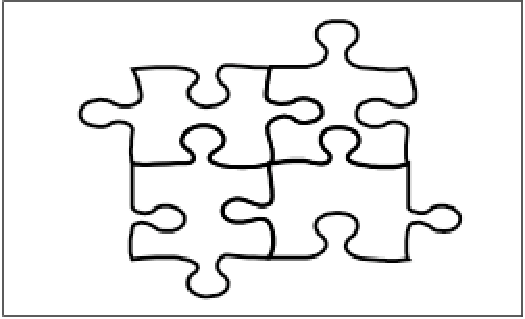
\includegraphics[height=4cm,width=6cm]{figs/fig1}
   \end{center}
   \caption{Old \jobim puzzle (end of the 20th century).}
   \label{fig:puzzle}
 \end{figure}


\begin{acknowledgements}
  \label{sec:acknowledgements}
This study makes use of data generated by the Blueprint Consortium, whose proprietary use was granted for exploratory analysis to the company Les Laboratoires Servier. A full list of the investigators who contributed to the generation of the data is available from \url{www.blueprint-epigenome.eu}.

We would also like to thank the BBC team within my company who implemented the RNASeq pipeline that was used to preprocess and curate both purified and bulk RNA datasets. The code used for that section can be found on \href{https://github.com/orgs/servier-github/repositories}{Servier-Github}.

\end{acknowledgements}


 \bibliography{jobim_proceedings}

 \appendix

\section{Model}
\subsection{The DeCoVart algorithm for deconvolution as constrained optimisation of a multivariate Gaussian convolution}
\label{subsubsec:contrained-optimisation}



\begin{property}[\textbf{matrix calculus}]
\label{pr:matrix-calculus-part-1}
Given two invertible squared matrices $\boldsymbol{A}$ and $\boldsymbol{B}$, with respective inverses $\boldsymbol{A}^{-1}$ and $\boldsymbol{B}^{-1}$, $A=\boldsymbol{A}(p)$ and $B=\boldsymbol{B}(p)$ being functions of a scalar variable $p$, the following properties hold:
\begin{multicols}{3}
\begin{enumerate}[label=(\alph*)]
\item $\frac{\partial \DET(\boldsymbol{A})}{\partial p}=\DET(\boldsymbol{A}) \Tr \left(\boldsymbol{A}^{-1} \frac{\partial \boldsymbol{A}}{\partial p} \right)$
\item $\frac{\partial \boldsymbol{U}\boldsymbol{A}\boldsymbol{V}}{\partial p} = \boldsymbol{U} \frac{\partial\boldsymbol{A}}{\partial p} \boldsymbol{V}$
\item $\frac{\partial \boldsymbol{A}^{-1}}{\partial p} = -\boldsymbol{A}^{-1} \frac{\partial\boldsymbol{A}}{\partial p} \boldsymbol{A}^{-1}$
\end{enumerate}
\end{multicols}
\end{property}

Notably, $\frac{\partial \log\left(\DET(\boldsymbol{A})\right)}{\partial p}= \Tr \left(\boldsymbol{A}^{-1} \frac{\partial \boldsymbol{A}}{\partial p} \right)$ using the chain rule applied to a logarithmic function (\textcolor{red}{alternative notation of the determinant of matrix: $\DET(\boldsymbol{A})=|\boldsymbol{A}|$}?). The function is well-defined, as $\boldsymbol{A}$ is positive-definite, hence its determinant is strictly positive. 

% Additionally, both the linear property of the derivative operator:$\frac{\partial c_1 \boldsymbol{A} + c_2 \boldsymbol{B}}{\partial p}=c_1 \frac{\partial \boldsymbol{A}}{\partial p} + c_2 \frac{\partial \boldsymbol{B}}{\partial p}$, $c_1$ and $c_2$ constants, and the multiplicative property:$\frac{\partial \boldsymbol{A} \boldsymbol{B}}{\partial p}= \boldsymbol{A}\frac{\partial \boldsymbol{B}}{\partial p} + \boldsymbol{B} \frac{\partial \boldsymbol{A}}{\partial p}$ holds similarly for matrices as for real valued functions.


\subsection{Parameter estimation with simplex constraints and the Levenberg–Marquardt algorithm}
\label{subsec:Levenberg–Marquardt}



%  \begin{tcolorbox}
% \begin{df}
% \label{def:positive-definite}
% A symmetric real matrix $\boldsymbol{A}$ of rank $G$ is said to be \textit{positive-definite} if $\boldsymbol{x}^\top \boldsymbol{A} \boldsymbol{x} > 0$ for all non-zero vectors $\boldsymbol{x}$ in $\mathbb{R}^G$.
% \end{df}
% \end{tcolorbox}

% \begin{tcolorbox}
% \begin{property}
% \label{pr:multivariate-affine-transformation}
% The two following properties hold for a multivariate Gaussian distribution:
% \begin{itemize}
%     \item if $\boldsymbol{X} \sim \mathcal{N}_G( \mu, \boldsymbol{\Sigma})$, then $p\boldsymbol{X}$, with $p$ a constant, follows itself a multivariate Gaussian distribution:
%     $p\boldsymbol{X} \sim \mathcal{N}_G (p \mu, p^2 \Sigma)$
    
%     \item given two independent random vectors $\boldsymbol{X_1} \sim \mathcal{N}_G(\mu_1, \boldsymbol{\Sigma_1})$ and  $\boldsymbol{X_2} \sim \mathcal{N}_G(\mu_2, \boldsymbol{\Sigma_2})$ of same size $G$ following a multivariate Gaussian distribution, then the random variable $\boldsymbol{X_1} + \boldsymbol{X_2}$ follows itself a multivariate Gaussian distribution: $X + Y \sim \mathcal{N}_G (\mu_1 + \mu_2, \boldsymbol{\Sigma_1} + \boldsymbol{\Sigma_2})$. We can be use the characteristic function of a multivariate Gaussian distribution to show this result.
    
%     By induction, this property generalises to the sum of $J$ independent random vectors of same size $G$, yielding $\sum_{j=1}^J \boldsymbol{X_j} \sim \mathcal{N}_G(\sum_{j=1}^J \mu_j, \sum_{j=1}^J \boldsymbol{\Sigma_j})$
% \end{itemize}
% \end{property}
% \end{tcolorbox}

\end{document}
